\documentclass[11pt,a4paper]{report}

\usepackage[english,italian]{babel}
\usepackage[T1]{fontenc}
\usepackage[utf8]{inputenc}
\usepackage{times}
\usepackage{hyperref}
\usepackage{titlesec}
\usepackage{amssymb,amsmath}
\usepackage[titles]{tocloft}
\usepackage{appendix}
\hypersetup{%
    pdfborder = {0 0 0}
}
\usepackage{graphicx}
\usepackage[svgnames]{xcolor} % Required to specify font color
\usepackage{eurosym}

\usepackage{titlesec}
\titleformat{\chapter}[hang] 
{\normalfont\huge\bfseries}{\chaptertitlename\ \thechapter.}{1em}{} 

\newcommand*{\plogo}{\fbox{$\mathcal{PL}$}} % Generic publisher logo
\usepackage{listings}
\usepackage{fancyhdr}

\usepackage{ragged2e}

\setlength{\voffset}{-0.5in}
\setlength{\topmargin}{-0.2in}
\setlength{\textheight}{240mm}
\setlength{\textwidth}{142mm}
\setlength{\evensidemargin}{0.3in}
\setlength{\oddsidemargin}{0.3in}

\begin{document}

\begin{titlepage}
\begin{center}
  \bfseries
  \huge UNIVERSITÀ DEGLI STUDI DI PADOVA
  \vskip-.1in
  \rule{\textwidth}{1.5pt}
  \vskip.1in
  \textsc{\LARGE Scuola di Scienze}
  \vskip.2in
  
\includegraphics[scale=.2]{images/logo-unipd}
  \vskip.25in
  \large CORSO DI LAUREA IN INFORMATICA
  \vskip.7in
  \Large PROGETTO \vskip.1in DI
  \vskip.1in
  \LARGE BASI DI DATI
  \vskip.7in
  \emph{\huge ValleVerde Tennis Club}
\end{center}

\vskip1in
\hskip.2\textwidth
\begin{minipage}{.75\textwidth}
  \begin{flushleft}
    \bfseries\large \par \emph{Marco Leorato Matricola: 1006028}
    \bfseries\large \par \emph{Federico Silvio Busetto Matricola:1026925}
  \end{flushleft}
\end{minipage}

\vskip0.9in
\centering
\bfseries
\Large ANNO ACCADEMICO 2014-2015
\end{titlepage}

\pagestyle{empty}
\newpage

\tableofcontents
\newpage
\listoffigures
\clearpage


%----------------------------------------------------------------------------------------
%	CONSTANTS
%----------------------------------------------------------------------------------------

\newcommand{\authorName}{Marco Leorato - Federico Silvio Busetto}

%----------------------------------------------------------------------------------------
%	HEADER FORMAT
%----------------------------------------------------------------------------------------

\fancyhf{}
\fancyhead[RE]{\small\scshape\nouppercase{\leftmark}}
%\fancyhead[LO]{\small\scshape\nouppercase{\rightmark}}
\fancyhead[LE,RO]{\small\thepage}
%\lhead{\rightmark}
\rhead{\leftmark}

\fancypagestyle{plain}{\fancyfoot[RO,LE]{\thepage}}

\rfoot{\thepage}

\fancyfoot[RO, LE]{\thepage}
\pagestyle{fancy}

\setlength{\parindent}{0pt}


%----------------------------------------------------------------------------------------
%	CONTENT
%----------------------------------------------------------------------------------------

\selectlanguage{english}%
\begin{abstract}
\justify
Il \textit{Tennis Club Valleverde} offre ai suoi soci la possibilità di praticare il loro sport preferito in un ambiente immerso nella natura. \\
Tra i servizi offerti dal Club, spicca la scuola Tennis, attiva in tutto il periodo dell’anno, nella quale vari istruttori sono a  disposizione dei soci che desiderano migliorare la loro tecnica di gioco tramite lezioni individuali oppure partecipando a corsi collettivi. \\
Ai soci è inoltre offerta la possibilità di poter giocare delle partite libere tra loro, scegliendo tra una vasta gamma di campi in base alla superficie che più si adatta ai loro gusti, prenotando comodamente online. \\
Per gestire questi servizi, il Tennis Club Valleverde si avvale di una base di dati associata ad un’applicazione web. \\
Le operazioni tipiche sono la creazione e la modifica di record anagrafici dei soci, la gestione dei campi e delle relative prenotazioni (evitando sovrapposizioni tra lezioni individuali, corsi e partite libere).
\end{abstract}

\section{Analisi dei Requisiti}
 %include abstract
\chapter{Progettazione Concettuale} 

\section{Lista delle Classi}
\begin{description}
\item[PERSONA:] rappresenta una generica persona fisica all’interno del Tennis Club
\begin{itemize}
\item CodFiscale: \textit{string} \hfill 
\item Nome: \textit{string}  \hfill 
\item Cognome: \textit{string}  \hfill 
\item Sesso: \textit{enum\{“Maschio”, “Femmina”\}}  \hfill 
\item DataNasc: \textit{date}  \hfill 
\item LuogoNasc: \textit{string}  \hfill 
\item Telefono: \textit{string}  \hfill 
\item Mail: \textit{string}  \hfill 
\end{itemize}
Chiave primaria: \underline{CodFiscale} \hfill \\

Viene definita una partizione in due sottoclassi specifiche, di seguito riportate:
\item[ISTRUTTORE:] modella un istruttore, cioè una persona che tiene un corso
\begin{itemize}
\item Qualifica: \textit{string} \hfill 
\item Retribuzione: \textit{int} \hfill 
\item DataAssunzione: \textit{date} \hfill 
\end{itemize}
\item[SOCIO:] modella un socio, cioè una persona non istruttore, che frequenta il Tennis Club ValleVerde
\begin{itemize}
\item DataIscrizione: \textit{date} \hfill 
\item Livello: \textit{enum\{'Principiante', 'Intermedio', 'Esperto'\}} \hfill 
\end{itemize}
\item[ACCOUNT:] modella un account posseduto da una persona del Tennis Club
\begin{itemize}
\item UserName: \textit{string} \hfill 
\item Admin: \textit{bool} \hfill 
\item Hash: \textit{string} \hfill 
\end{itemize}
Chiave primaria (definita come identificatore esterno): \underline{CodFiscale} \hfill 
\item[CORSO:] modella un generico corso tenuto all’interno della scuola Tennis del Tennis Club
\begin{itemize}
\item CodCorso: \textit{int} \hfill
\item NomeCorso: \textit{string} \hfill
\item TipoCorso: \textit{enum\{‘Principiante’,’Intermedio’,’Avanzato’\}} \hfill
\item Attivo: \textit{bool} \hfill
\end{itemize}
Chiave primaria: \underline{CodCorso} \hfill 
\item[LEZIONE:] rappresenta una lezione di un corso
\begin{itemize}
\item CodLezione: \textit{int} \hfill 
\end{itemize}
Chiave primaria: \underline{(CodCorso,CodLezione)} \hfill 
\item[CAMPO:] modella un campo da Tennis
\begin{itemize}
\item CodCampo: \textit{int} \hfill 
\item TipoSup: \textit{enum\{‘Terra rossa’, ‘Erba sintetica’, ‘Playit’\}}
\end{itemize}
Chiave primaria: \underline{CodCampo} \hfill 
\item[PRENOTAZIONE:] modella una prenotazione di un campo
\begin{itemize}
\item Data: \textit{date} \hfill 
\item Ora: \textit{int} \hfill  
\end{itemize}
Chiave primaria: \underline{(CodCampo,Data,Ora)} \hfill 
\end{description}

\section{Lista delle Associazioni}

\begin{itemize}
\item \textsc{Persona - Account:} \textbf{Possiede}
\begin{itemize}
\item Ogni persona possiede un solo account. Ogni account è posseduto da una sola persona.
\item Molteplicità 1:1
\item Totalità: Totale in entrambi i sensi.
\end{itemize}

\item \textsc{Persona – Prenotazione:} \textbf{Fa}
\begin{itemize}
\item Una persona fa zero o più prenotazioni, ogni prenotazione viene fatta da una sola persona.
\item Molteplicità: 1:N
\item Totalità: Totale da Prenotazione verso Persona, parziale da Persona verso Prenotazione.
\end{itemize}

\item \textsc{Istruttore – Corso:} \textbf{Tiene}
\begin{itemize}
\item Un istruttore tiene zero o più corsi, ogni corso è tenuto da un solo istruttore.
\item Molteplicità: 1:N
\item Totalità: Parziale da Istruttore verso Corso, totale da Corso a Istruttore
\end{itemize}
\item \textsc{Socio - Corso:} \textbf{IscrittoCorso}
\begin{itemize}
\item Un socio è iscritto a zero o più corsi, un corso ha zero o più soci iscritti
\item Molteplicità: 1:N
\item Totalità: Parziale ambo i lati
\end{itemize}
\item \textsc{Corso - Lezione:} \textbf{CompostoDa}
\begin{itemize}
\item Un corso è composto da zero o più lezioni, zero o più lezioni compongono un corso.
\item Molteplicità: 1:N
\item Totalità: Parziale da Corso a Lezione, totale da Lezione a Corso
\end{itemize}
\item \textsc{Prenotazione - Campo:} \textbf{Riguarda}
\begin{itemize}
\item Una prenotazione riguarda un campo, ogni campo ha zero o più prenotazioni.
\item Molteplicità: 1:1
\item Totalità: Totale da Prenotazione a Campo, parziale da Campo a Prenotazione 
\end{itemize}
\item \textsc{Prenotazione – Lezione:} \textbf{Fissa}
\begin{itemize}
\item Una prenotazione fissa zero o una lezione, una lezione viene fissata da una prenotazione. Possono esserci lezioni per le quali non è ancora stata effettuata una prenotazione.
\item Molteplicità: 1:1
\item Totalità: Parziale ambo i lati
\end{itemize}
\end{itemize}

\section{Descrizione della Gerarchia}
L'unica gerarchia presente nello schema concettuale riguarda la superclasse \textit{Persona} che si divide nelle due sottoclassi specializzate \textit{Istruttore} e \textit{Socio}.\\

Tale generalizzazione è \textit{Totale} in quanto ogni occorrenza di \textit{Persona} è anche occorrenza di \textit{Istruttore} o di \textit{Socio} (ricordiamo che \textit{Persona} modella una persona fisica all'interno del Tennis Club).\\
La generalizzazione è inoltre \textit{esclusiva}, in quanto una \textit{Persona} rappresentata dalla superclasse non può essere contemporaneamente \textit{Socio} e \textit{Istruttore}.\\

Le due sottoclassi specializzate prevedono degli attributi propri per modellare gli istruttori (\textit{Qualifica}, \textit{Retribuzione} e \textit{DataAssunzione}) e i soci (\textit{DataIscrizione} e \textit{Livello}).

\section{Vincoli di Integrità aggiuntivi}
\section{Schema concettuale E-R}
\begin{figure}[H]
 \centering
  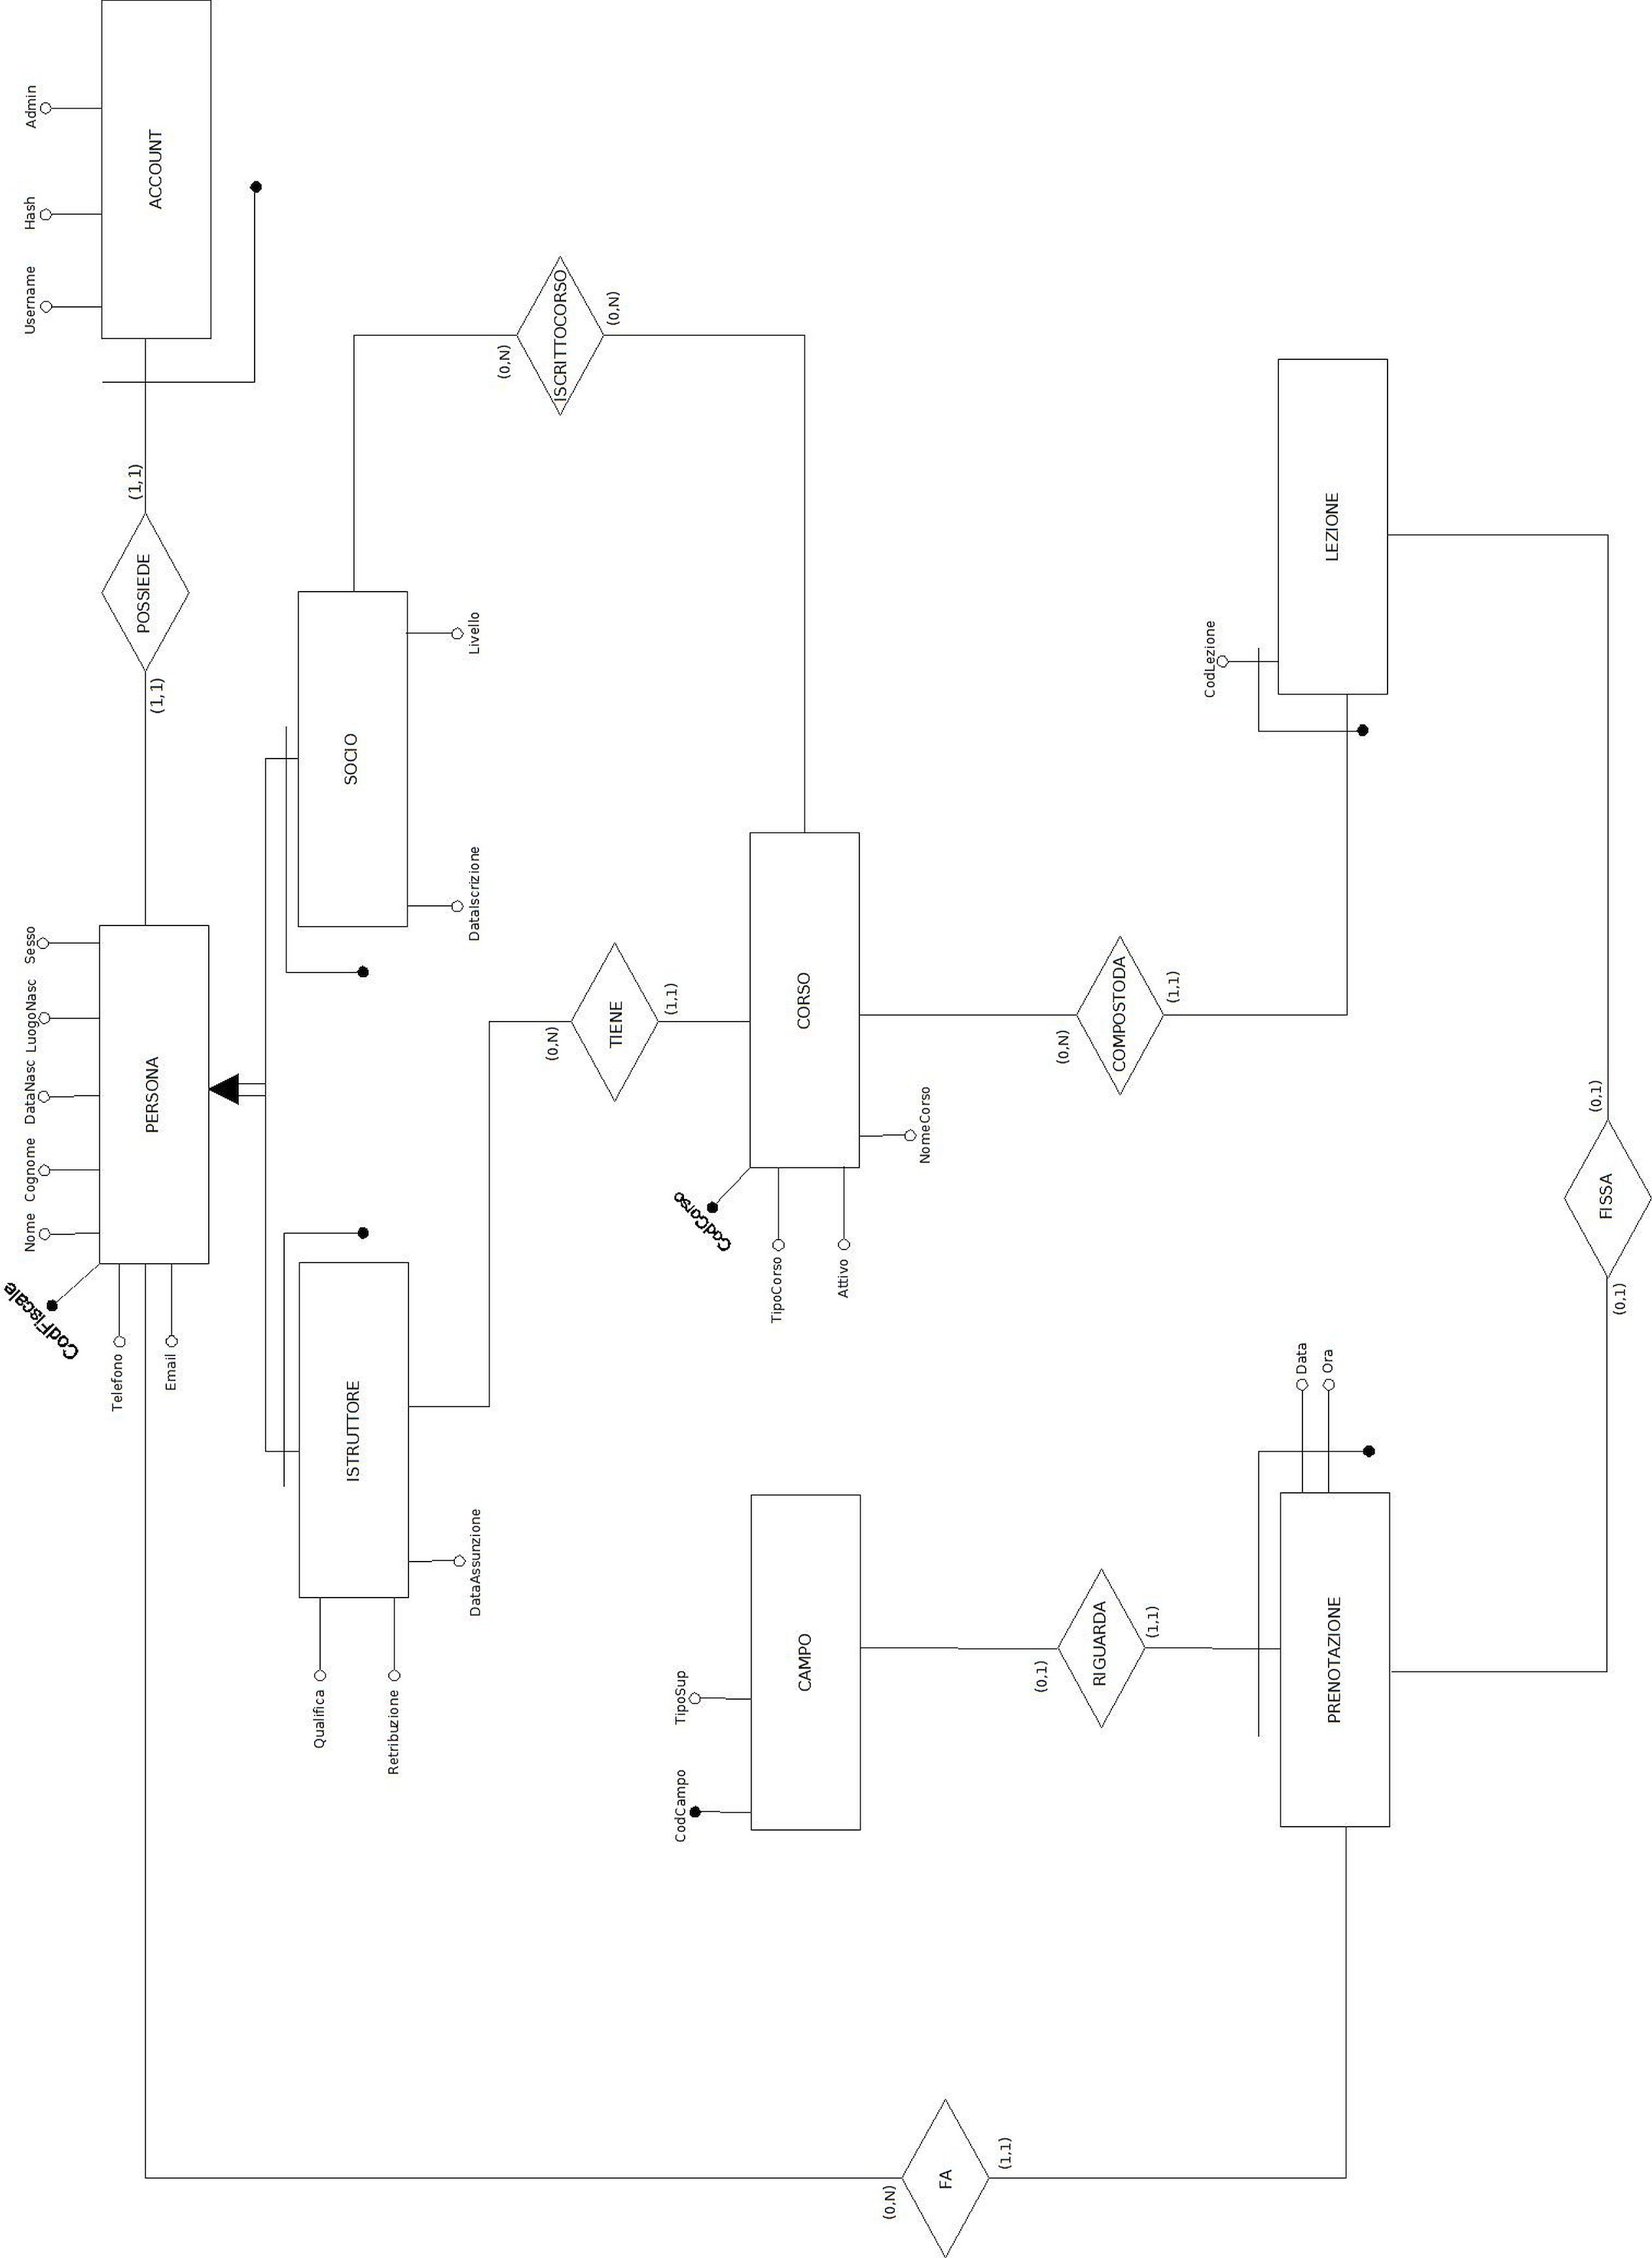
\includegraphics[width=\textwidth, height=\textheight]{Images/ER_FINALE.jpg}
\caption{Schema Concettuale E-R}
\end{figure} 
\chapter{Progettazione Logica} 

\section{Gerarchia}
La gerarchia della classe \textit{Persona} è stata implementata con partizionamento verticale visto che entrambe le sottoclassi \textit{Istruttore} e \textit{Socio} hanno degli attributi propri e considerato il fatto che sia la classe radice che le due sottoclassi hanno delle associazioni proprie.\\
Si è scelto di sostituire la generalizzazione con associazioni, in modo da evitare di avere attributi con valori nulli suul'entità genitore e di ridurre la dimensione delle entità figlie. 

\section{Descrizione testuale dello schema relazionale}
Le chiavi primarie vengono indicate come \underline{sottolineate}, mentre le chiavi esterne vengono marcate con un asterisco (*).\\

\begin{itemize}
\item \textsc{Persona}(\underline{\textbf{CodFiscale}}: string, \textbf{Nome} :string, \textbf{Cognome}: string, \textbf{DataNasc}: date,\\ \textbf{LuogoNasc}: string, \textbf{Telefono}: string,  \textbf{Mail}: string, \textbf{Sesso}: enum\{'Maschio', 'Femmina'\} ) 
\begin{itemize}
\item Tutti i campi di Persona sono implementati come NOT NULL (tranne telefono, perché facoltativo).
\end{itemize}

\item \textsc{Istruttore}(\underline{\textbf{CodFiscale}*}: string, \textbf{Qualifica}: string, \textbf{Retribuzione}: int, \textbf{DataAssunzione}: date)
\begin{itemize}
\item Tutti i campi sono NOT NULL tranne il campo \textit{Qualifica} che può essere vuoto.
\item \textit{Retribuzione} deve essere un valore positivo, maggiore di zero.
\end{itemize}

\item \textsc{Socio}(\underline{\textbf{CodFiscale}*}: string, \textbf{DataIscrizione}: date. \textbf{Livello}: enum\{'Principiante',\\'Intermedio','Esperto'\})  
\begin{itemize}
\item Tutti i campi sono NOT NULL.
\end{itemize}

\item \textsc{Account}(\underline{\textbf{CodFiscale}*} string, \textbf{UserName}: string, \textbf{Admin}: bool, \textbf{Hash}: string )
\begin{itemize}
\item Tutti i campi sono NOT NULL.
\item Il campo \textit{Admin} rappresenta i permessi e distingue un utente con permessi amministrativi (istruttore, 1) da un utente con permessi di default (socio, 0).
\item Il campo \textit{Hash} memorizza l'hash SHA1 della password associata all'account.
\end{itemize}

\item \textsc{Corso}(\underline{\textbf{CodCorso}*}: int, \textbf{NomeCorso}: string, \textbf{TipoCorso}: enum\{'Principiante',\\'Intermedio','Avanzato'\}, \textbf{Attivo}: bool, \textbf{CodFiscale}*: string)
\begin{itemize}
\item Tutti i campi tranne \textit{CodFiscale} sono NOT NULL. Vi possono essere corsi per il quale non v'è Istruttore.
\item Il campo \textit{Attivo} che determina se un corso è attivo, oppure no, è impostato di default a zero.
\end{itemize}
\item \textsc{Campo}(\underline{\textbf{CodCampo}}: int, \textbf{TipoSup}: enum\{'Terra Rossa','Erba Sintetica','PlayIt'\})
\begin{itemize}
\item Tutti i campi sono NOT NULL.
\end{itemize}

\item \textsc{Lezione}(\underline{\textbf{CodLezione}}: int, \underline{\textbf{CodCorso}*}: int )   
\item \textsc{IscrittoCorso}(\underline{CodCorso}*: int, \underline{\textbf{CodFiscale}*}: string) 
\begin{itemize}
\item Nuova tabella derivante dall'associazione \textit{IscrittoCorso}
\end{itemize}
\item \textsc{Prenotazione}(\textbf{CodCorso}*:int, \textbf{CodLezione}*: int, \textbf{CodFiscale}*: string, \underline{\textbf{CodCampo}*}: int, \underline{\textbf{Data}}: date, \underline{\textbf{Ora}}: tinyint)  
\begin{itemize}
\item I campi \textit{CodCorso}, \textit{CodLezione}, \textit{CodFiscale} possono essere NULL ma non tutti e tre contemporaneamente.
\end{itemize}
\end{itemize}

\section{Vincoli semantici non catturati dallo schema}
\section{Schema logico}
\begin{figure}[H]
 \centering
  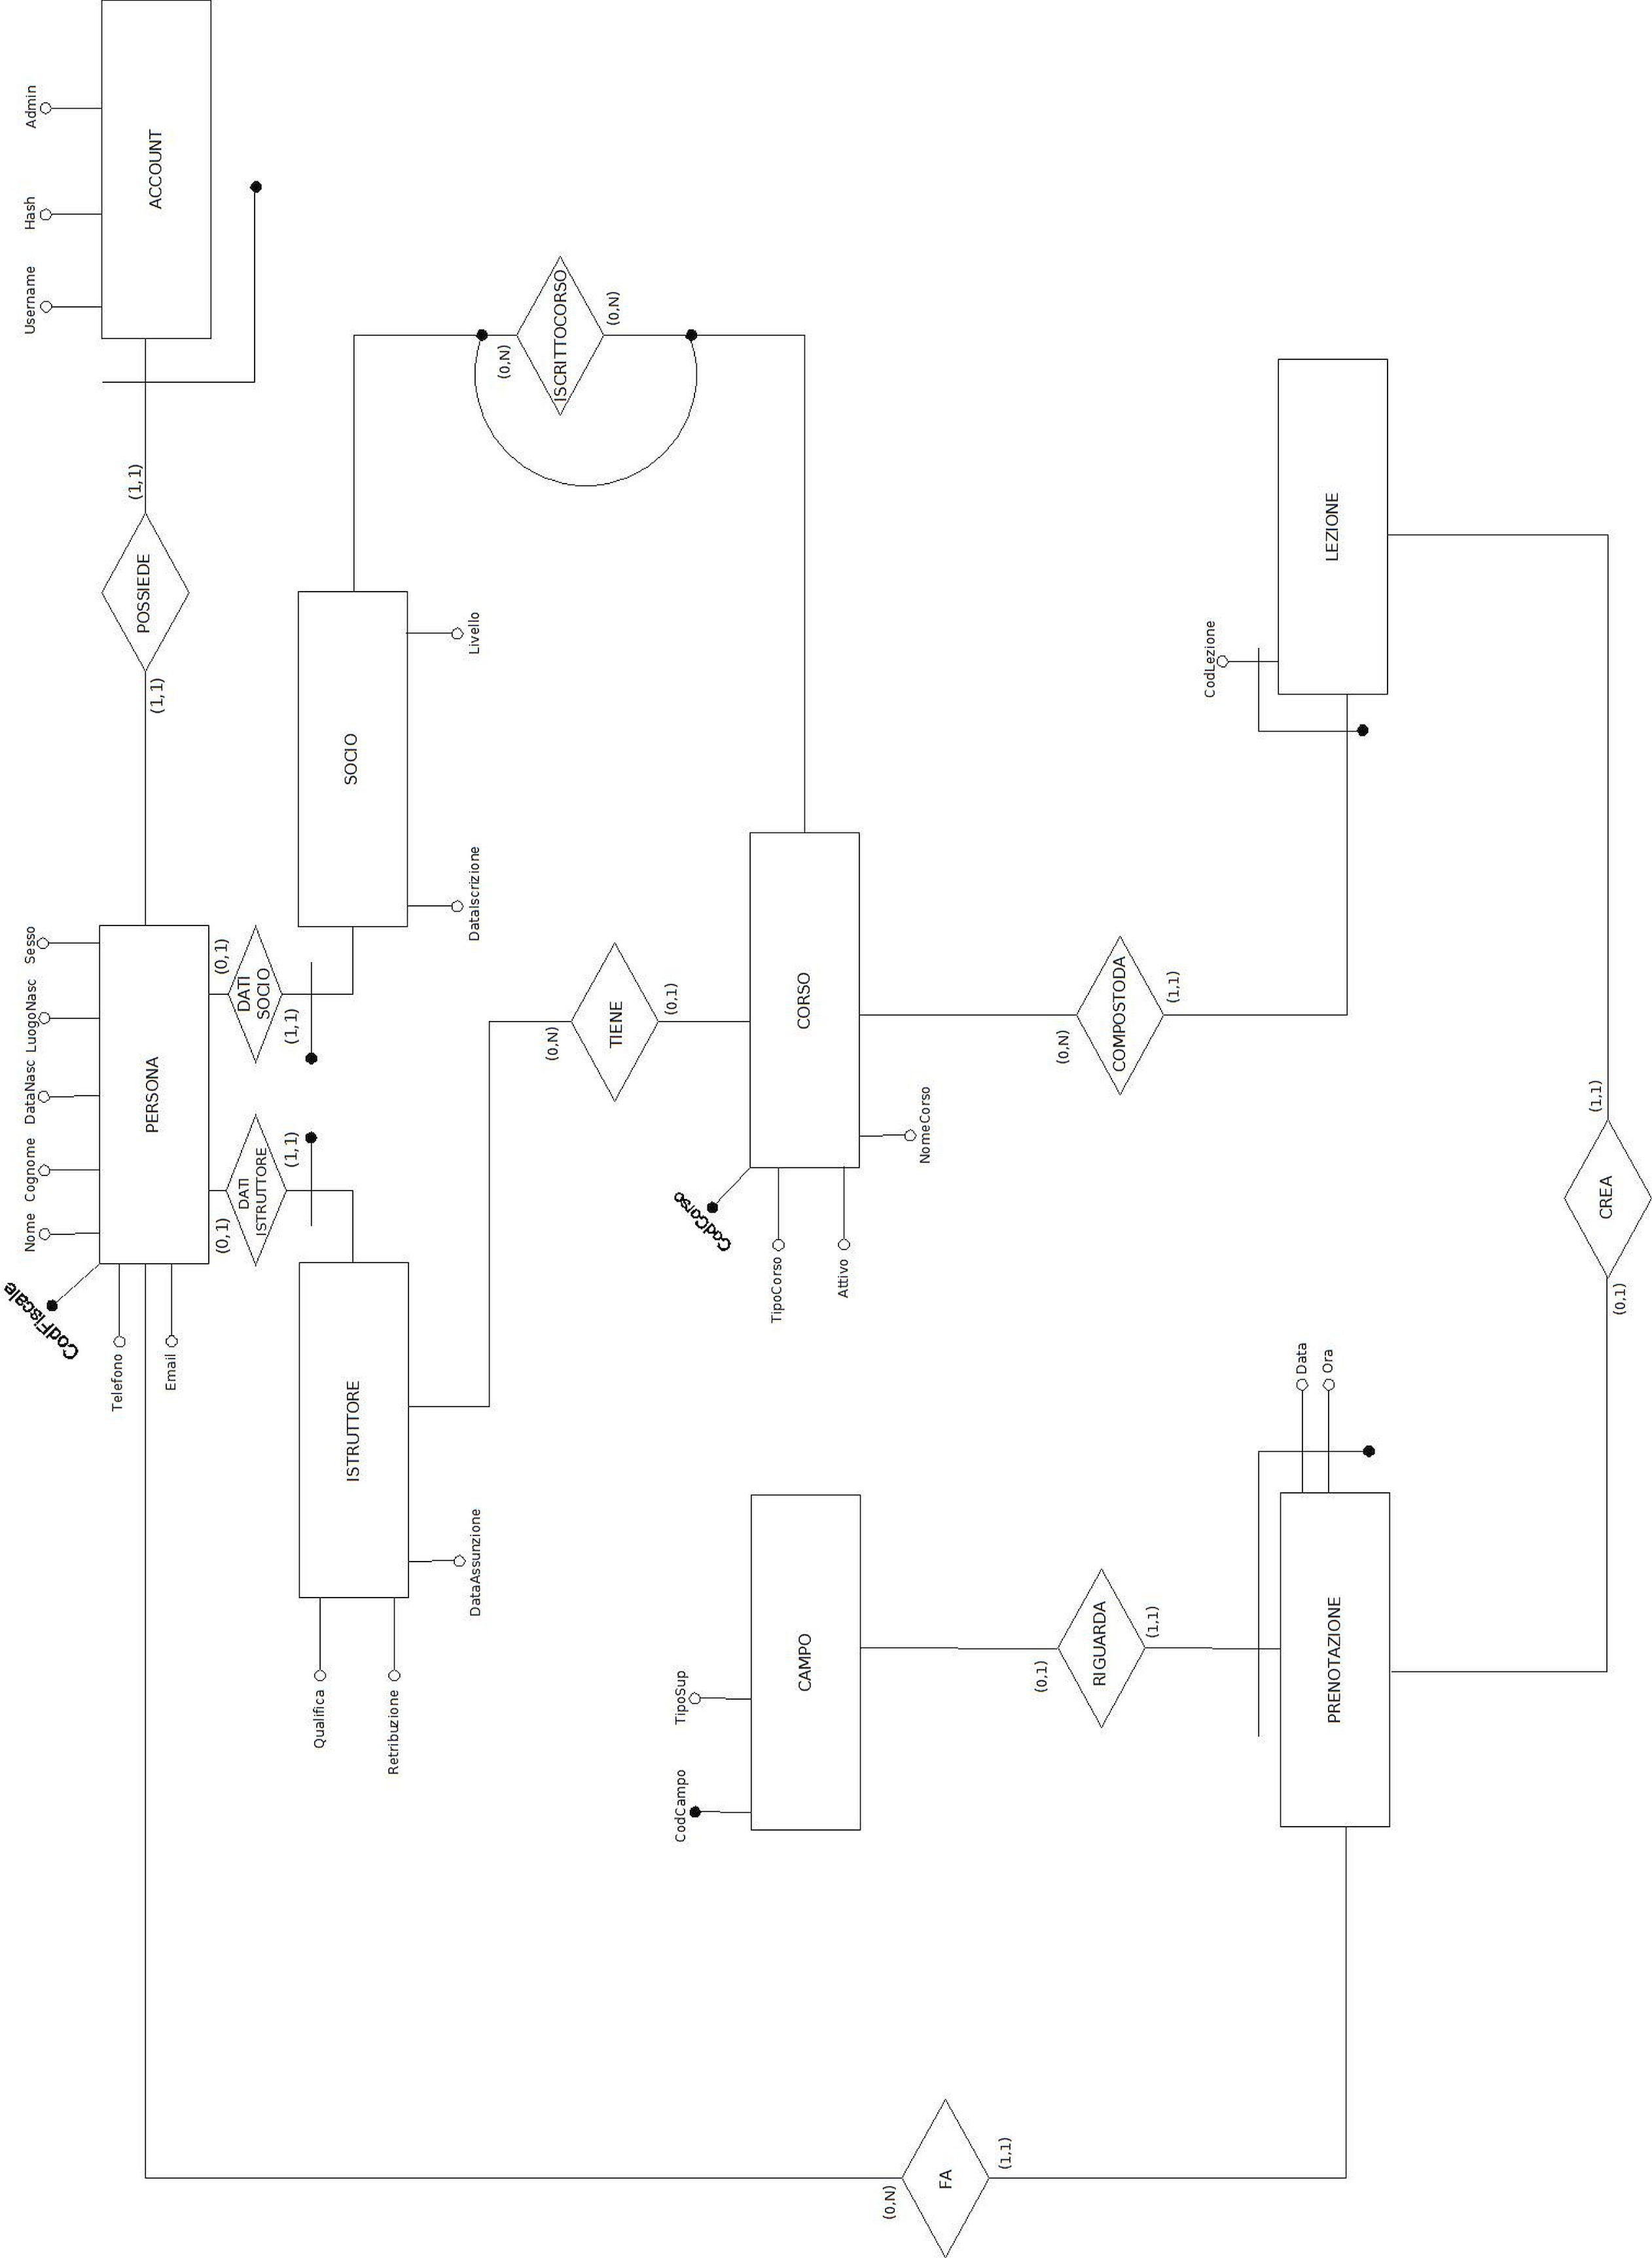
\includegraphics[width=\textwidth, height=\textheight]{images/LOGICO.jpg}
\caption{Lo Schema Concettuale E-R Ristrutturato}
\end{figure}
\chapter{Implementazione dello schema logico tramite DDL di MySQL} 
\lstinputlisting[language=SQL,firstline=1,lastline=95]{sql/DDL_Database.sql}
 %include schema logico e DDL SQL
\chapter{Query} 
L'interfaccia web utilizza varie query di servizio, di seguito vengono proposte alcune tra le piu' significative adattate a casi particolari.

\section{Query 1}

Recupera la lista di tutti i corsi con i nomi degli istruttori associati.\\

\lstinputlisting[language=SQL,firstline=1,lastline=3]{sql/Query.sql}

\section{Query 2}

Recupero le informazioni riguardanti il corso 4.\\

\lstinputlisting[language=SQL,firstline=5,lastline=9]{sql/Query.sql}

\section{Query 3}

Estrae le prenotazioni fatte dopo la data del 25 agosto 2015, mostrando per ognuna i dati dell'utente e della prenotazione.\\

\lstinputlisting[language=SQL,firstline=11,lastline=15]{sql/Query.sql}

\section{Query 4}
Restituisce, se c'e', una prenotazione per il campo 3 nella data 16-09-2015 alle ore 13.\\

\lstinputlisting[language=SQL,firstline=17,lastline=20]{sql/Query.sql}

\section{Query 5}
Recupero la lista delle lezioni del corso 2 e, se disponibili  anche le prenotazioni corrispondenti.\\

\lstinputlisting[language=SQL,firstline=22,lastline=26]{sql/Query.sql}

\section{Query 6}

Estrae le informazioni di tutti i corsi attivi ai quali l'utente e' iscritto, con nome e cognome del rispettivo istruttore.\\

\lstinputlisting[language=SQL,firstline=28,lastline=37]{sql/Query.sql}

\section{Query 7}

Mostra le prenotazioni dell'utente che visualizza la pagina alla data indicata.\\

\lstinputlisting[language=SQL,firstline=38,lastline=44]{sql/Query.sql}

\chapter{Trigger e Funzioni} 

\section{Trigger}

\subsection{InserimentoRetribuzione}
\lstinputlisting[language=SQL,firstline=98,lastline=110]{sql/DDL_Database.sql}

Il trigger esprime il vincolo semantico che la retribuzione di un'istruttore non possa essere un valore negativo (minore o uguale a zero). Nel caso lo sia, imposta una retribuzione base di 800 euro.
Questo trigger è dedicato alle operazioni di inserimento.

\subsection{AggiornaRetribuzione}
\lstinputlisting[language=SQL,firstline=112,lastline=124]{sql/DDL_Database.sql}

Trigger simile al precedente, utilizzato in caso di aggiornamento del campo retribuzione. Nel caso la retribuzione dell'istruttore venga impostata ad un valore negativo, viene ripristinato il vecchio valore.

Sono stati necessari due trigger visto che MySQL non permette di definire trigger su condizioni multiple.

\subsection{CorsoAttivoIns}
\lstinputlisting[language=SQL,firstline=126,lastline=137]{sql/DDL_Database.sql}

Imposta un corso come non attivo se manca il codice fiscale dell'istruttore che lo tiene. Vale per l'inserimento di nuovi corsi.

\subsection{CorsoAttivoUpd}

\lstinputlisting[language=SQL,firstline=139,lastline=150]{sql/DDL_Database.sql}

Imposta un corso come non attivo se manca il codice fiscale dell'istruttore che lo tiene. Vale per l'aggiornamento dei corsi.

\subsection{CorsoAttivoElim}

\lstinputlisting[language=SQL,firstline=152,lastline=166]{sql/DDL_Database.sql}

Come i trigger precedenti, si occupa di impostare il campo \textit{Attivo} di un corso a false (0) se viene eliminato l'istruttore che tiene quel corso.

\section{Funzioni}

\subsection{ControlloPrenotazione}

\lstinputlisting[language=SQL,firstline=173,lastline=193]{sql/DDL_Database.sql}

\subsection{ControlloPrenotazioneCorso}

\lstinputlisting[language=SQL,firstline=196,lastline=221]{sql/DDL_Database.sql}

\subsection{PossoIscrivermi}

\lstinputlisting[language=SQL,firstline=224,lastline=266]{sql/DDL_Database.sql} %include view,funzioni,trigger,procedure
\chapter{Interfaccia Web} 
 
\section{Descrizione interfaccia}

Per interagire con il database e' stata sviluppata un'interfaccia web.

\subsection{Layout}
Si e' optato per un classico layout cosi' strutturato:

\begin{itemize}
\item Spazio per titolo e logo del sito
\item Una barra informativa che indica la posizione dell'utente all'interno del sito e alla destra un link alla pagina di login.
\item Un menu' di navigazione laterale personalizzato in base ai permessi dell'utente che effettua il login.
\item Un box centrale con il contenuto della pagina.
\end{itemize}

\subsection{CSS}

Gli aspetti grafici basilari per il rendering delle pagine web vengono gestiti tramite CSS, particolare attenzione e' stata dedicata alla scelta dei colori per permettere una navigazione del sito anche a persone con problemi di vista.

\section{Descrizione delle pagine}

\section{Funzioni}
Il file \textit{phpfunctions.php} contiene le funzioni base utilizzate da tutte le altre pagine php.

\subsection{connessione}
Effettua la connessione al server.

\subsection{chiusura}
Chiude la connessione al server, quando necessario.

\subsection{loginlink}
Gestisce i link per il login della barra informativa orizzontale distinguendo se l'utente e' loggato o meno.

\subsection{menu}

Genera il menu' verticale laterale.

\subsection{addadmin.php}

Aggiunge un nuovo istruttore che avra' privegi amministrativi.

\subsection{adduser.php}

Aggiunge un nuovo utente con privilegi di default.

\subsection{corsi.php}

Pagina che usa un socio per visualizzare i corsi ai quali e' iscritto e accedere alle informazioni dei corsi.

\subsection{gcorsi.php}

Pagina che usa l'amminsitratore per visualizzare tutti i corsi, aggiungerne di nuovi e accedere alle informazioni dei corsi.

\subsection{gestiscicorso.php}

Visualizza tutte le informazioni del corso, dando accesso alle pagine per vedere gli iscritti, aggiungere le nuove prenotazioni ai campi per le lezioni del corso, modificare le informazioni del corso o cancellarlo. Solo lato admin.

\subsection{gprenotazioni.php}

Permette agli istruttori di vedere, fare ricerche e cancellare prenotazioni.

\subsection{gutenti.php}

Gestione degli utenti, permette agli istruttori di vedere e fare ricerche sugli utenti. Accedere ai dettagli degli utenti ed aggiungere un nuovo account utente o amministratore. 

\subsection{index.php}

La pagina principale del corso.

\subsection{informazionicorso.php}

Permette all'utente di visualizzare informazioni dettagliate di un corso (tra le quali anche le lezioni prenotate), iscriversi in base al suo livello e cancellare l'iscrizione ai corsi.

\subsection{iscritticorso.php}

Visualizza le persone iscritte ad un corso e permette agli istruttori la cancellazione delle loro iscrizioni.

\subsection{login.php}

Gestisce il login.

\subsection{logout.php}

Effettua il logout e rimanda all'index.

\subsection{modadmin.php}

Visualizza informazioni sugli istruttori e permette di modificarle agli istruttori.

\subsection{modificacorso.php}

Permette agli istruttori di modificare le informazioni dei corsi.

\subsection{moduser.php}

Permette agli istruttori di modificare le informazioni dei soci.

\subsection{prenotalezione.php}

Permette di prenotare un campo per una nuova lezione di un corso.

\subsection{prenotazione.php}

In base se l'utente e' socio oppure istruttore permette:
\begin{itemize}
\item A soci e istruttori di vedere le proprie prenotazioni e le prossime lezioni dei corsi.
\item A soci e istruttori di effettuare e rimuovere prenotazioni personali. 
\item Ai soci, vedere le prenotazioni ai corsi ai quali e' iscritto
\item Agli istruttori, di vedere le prenotazioni ai campi delle prossime lezioni dei corsi tenuti.
\end{itemize}

\subsection{utenti.php}

Permette di vedere e modificare le proprie informazioni (tranne la data di assunzione/iscrizione) e cancellare l'account. %tutta la parte web
\chapter{Considerazioni Finali} 

\section{Note per l'installazione}

Per permettere un'agevole navigazione nel progetto sono stati aggiunti due account forniti di diverso livello di permessi. \\
\begin{itemize}
\item E' possibile l'accesso all'account  di un utente socio generico con permessi di default usando le credenziali:
\begin{itemize}
\item \textbf{\textit{Username:}} user
\item \textbf{\textit{Password:}} user
\end{itemize} 

\item E' possibile l'accesso all'account di un utente istruttore generico con permessi \\ amministrativi usando le credenziali:
\begin{itemize}
\item \textbf{\textit{Username:}} admin
\item \textbf{\textit{Password:}} admin
\end{itemize} 
\end{itemize}

Sempre per comodita' di valutazione, e' possibile l'accesso come un qualsiasi utente visto che le password coincodono coincidono con lo username dell'account.

\section{Licenza}
Tutto il codice sorgente in PHP, CSS, SQL compreso quello di questa relazione \LaTeX  è da intendersi come rilasciato sotto \textit{GPLv3}\\
\url{http://choosealicense.com/licenses/gpl-3.0/} 
 . \\ Il file risultante dalla compilazione del sorgente \LaTeX è da considerarsi come rilasciato sotto licenza \textit{CC BY-SA 4.0}\\ \url{http://creativecommons.org/licenses/by-sa/4.0/} 

\section{Strumenti utilizzati}
Per la realizzazione degli schemi è stato utilizzato il software \textbf{Gnome Dia}, come strumenti di collaborazione son stati utilizzati un repository su \textit{github} e una cartella su cloud presso il servizio di cloud storage \textit{mega.nz}. %eventuali considerazioni finali

%\appendix

%\input{glossario}
\end{document}